% !TeX spellcheck = fr_FR
\chapter{Chapitre 8 : Backend}

Ce chapitre présente l'architecture backend qui alimente l'application: structure par \textit{blueprints} Flask\citeref{ref:flask_docs}, sérialisation, requêtage optimisé, endpoints majeurs (données, recherche, statistiques, rapports) et services dédiés (routes).

Le \textbf{chapitre 10} traitera exclusivement de l'authentification (flux, 2FA, emails), et le \textbf{chapitre 11} proposera un audit sécurité global (CSP, rate-limiting, surfaces d'attaque, secrets, etc.).

\section{Architecture générale}
\subsection*{Initialisation de l'application}

Le fichier \texttt{backend/app.py} centralise la configuration (deux \textit{binds} SQLAlchemy: \texttt{stops\_db} et \texttt{auth\_db}), les extensions (SQLAlchemy, CSRF, Limiter, Talisman, Migrate) et l'enregistrement des blueprints.

\paragraph{Décisions structurantes}
\begin{itemize}
  \item \textbf{Séparation des données} \texttt{stops\_db} vs \texttt{auth\_db}: isolement sécurité et privilèges distincts (Chap.~10), tout en simplifiant les migrations.
  \item \textbf{Extensions par défaut} activées dès l'init: \texttt{CSRF} (protection formulaire/AJAX), \texttt{Limiter} (défense anti-abus), \texttt{Talisman} (en-têtes de sécurité), \texttt{Migrate} (évolution du schéma sans downtime).
  \item \textbf{Organisation par domaines} via blueprints: \texttt{data}, \texttt{search}, \texttt{stats}, \texttt{reports}, \texttt{problems}, \texttt{auth}. Chaque route reste courte et testable.
\end{itemize}

\subsection*{Modèles et sérialisation}

Les tables applicatives sont décrites dans \texttt{backend/models.py} (cf. Chap.~7 pour le schéma). La sérialisation cohérente d'un \texttt{Stop} en JSON est gérée par \texttt{backend/serializers/stops.py}.

\paragraph{Contrat JSON minimal d'un \texttt{Stop}}
\begin{itemize}
  \item \textbf{Identité}: \texttt{id}, \texttt{sloid}, \texttt{osm\_node\_id}
  \item \textbf{Typage}: \texttt{stop\_type} (\texttt{matched|unmatched|osm}), \texttt{match\_type} (\texttt{auto|manual})
  \item \textbf{Position}: \texttt{atlas\_lat/lon} avec \textit{fallback} OSM si manquant; \texttt{osm\_lat/lon}
  \item \textbf{Métadonnées}: \texttt{distance\_m}, \texttt{uic\_ref}, \texttt{osm\_node\_type}
  \item \textbf{Invariants}: toujours renvoyer des coordonnées exploitables pour le rendu; éviter les \texttt{JOIN} au point de clic (détails chargés à la demande)
\end{itemize}

\section{Blueprints et endpoints}
Nous structurons l'API par \textit{domaine} pour garder des fichiers courts, testables et lisibles.

\subsection{Données: \texttt{/api/data}}

\textbf{Fichier}: \texttt{backend/blueprints/data.py}. Endpoint principal pour alimenter la carte.

\textbf{Rôle}
\begin{itemize}
  \item Filtrer par \textbf{fenêtre cartographique} (bbox), \textbf{types de transport}, \textbf{opérateurs}, \textbf{lignes/directions}
  \item Paginer et renvoyer un \textbf{JSON compact} prêt à dessiner
  \item \textbf{Rate limiting}: \texttt{30/min}
\end{itemize}

\textbf{Pourquoi c'est rapide}
\begin{itemize}
  \item Schéma de Chap.~7: une ligne \texttt{stops} suffit pour un marqueur (pas de \texttt{JOIN})
  \item Filtrage \textit{SARGable} sur indexes lat/lon ATLAS et OSM
  \item Sérialisation minimale et pagination systématique
\end{itemize}

\subsection{Recherche et matches manuels}

\textbf{Fichier}: \texttt{backend/blueprints/search.py}. Recherches textuelles et \textit{matches} manuels.

\textbf{Endpoints clés}
\begin{itemize}
  \item \texttt{/api/search}: recherche par nom, opérateur, UIC
  \item \texttt{/api/top\_matches}: tri par distance croissante selon filtres actifs
  \item \texttt{/api/manual\_match} (POST): crée un \textit{match} ATLAS \(\leftrightarrow\) OSM, avec option de persistance
\end{itemize}

\textbf{Persistance des \textit{matches}}
\begin{itemize}
  \item Marque les deux entrées comme \texttt{matched} avec \texttt{match\_type = manual}
  \item Si demandé, enregistre des marqueurs persistants pour survivre aux ré-imports (cf. Chap.~7)
\end{itemize}

\subsection{Statistiques: \texttt{/api/global\_stats}}

\textbf{Fichier}: \texttt{backend/blueprints/stats.py}. Statistiques agrégées avec \textbf{cache LRU}.

\textbf{Choix de conception}
\begin{itemize}
  \item Clé de cache \textit{canonique} construite à partir des filtres triés
  \item Capacité bornée (50) avec éviction LRU et verrou léger pour la concurrence
  \item \textbf{Rate limiting} \texttt{30/min} pour éviter le sur-calcul
\end{itemize}

\subsection{Rapports: \texttt{/api/generate\_report}}

\textbf{Fichier}: \texttt{backend/blueprints/reports.py}. Génération PDF/CSV (\texttt{pdfkit}).

\textbf{Principes}
\begin{itemize}
  \item \textbf{Auth requise} et \textbf{quotas} (\texttt{20/jour}) pour limiter l'abus
  \item Requêtes \textbf{optimisées par colonne}: seules les colonnes nécessaires sont sélectionnées
  \item Deux chemins: rendu template HTML \(\rightarrow\) PDF ou export CSV avec en-têtes adaptés
\end{itemize}

\subsection{Problèmes et persistance}

\textbf{Fichier}: \texttt{backend/blueprints/problems.py}. Consultation, filtrage, tri, et persistance des solutions/notes. (Chap.~7 détaille la persistance côté import et modèle; ici nous couvrons l'API.)

\textbf{Capacités}
\begin{itemize}
  \item \texttt{/api/problems}: liste paginée (tri par priorité puis distance)
  \item \texttt{/api/problems/stats}: totaux \texttt{résolus/non résolus} par type
  \item \texttt{/api/save\_solution} et \texttt{/api/save\_note/<note\_type>}: écriture simple
  \item \texttt{/api/make\_solution\_persistent} et \texttt{/api/make\_note\_persistent/<note\_type>}: persistance entre ré-imports
\end{itemize}

\section{Requêtage partagé et optimisation}

\subsection*{QueryBuilder et FilterBuilder}

\textbf{Fichier}: \texttt{backend/query\_builder.py}. Centralise les patrons de filtres (type de transport, type de nœud, opérateurs ATLAS, routes) et applique des options de chargement si nécessaire.

\textbf{Filtres pris en charge}
\begin{itemize}
  \item \textbf{Transport}: \texttt{station}, \texttt{platform}, \texttt{stop\_position}, etc. (via sous-requêtes sur \texttt{osm\_nodes})
  \item \textbf{Opérateurs ATLAS}: filtre sur \texttt{atlas\_stops.operator}
  \item \textbf{Routes/directions}: via \texttt{routes\_and\_directions} pour alimenter la UI
\end{itemize}

\textbf{Invariants de composition}
\begin{itemize}
  \item Les conditions de transport sont agrégées par \texttt{OR}, puis combinées avec le reste par \texttt{AND}
  \item Paramètres homogènes et stables côté API: \texttt{transport\_types}, \texttt{operators}, \texttt{bbox}, etc.
\end{itemize}

\subsection*{Services de routes}

\textbf{Fichier}: \texttt{backend/services/routes.py}. Service \texttt{get\_stops\_for\_route(route\_id, direction)} en SQL brut sur \texttt{routes\_and\_directions}.

\textbf{Points clés}
\begin{itemize}
  \item \textbf{Recherche tolérante}: correspondance par \texttt{LIKE} sur \texttt{osm\_route\_id}, \texttt{atlas\_route\_id} ou \texttt{atlas\_line\_name}
  \item \textbf{Fallback} de normalisation (ex.: \texttt{-j24} \(\rightarrow\) \texttt{-jXX}); récursif tant que l'ID se simplifie
  \item \textbf{Charge minimale}: sélection d'une ligne \texttt{LIMIT 1} indexée, et désérialisation JSON côté Python
\end{itemize}

\section{Diagrammes de flux}

\subsection*{Flux d'une requête cartographique}

\begin{figure}[H]
  \centering
  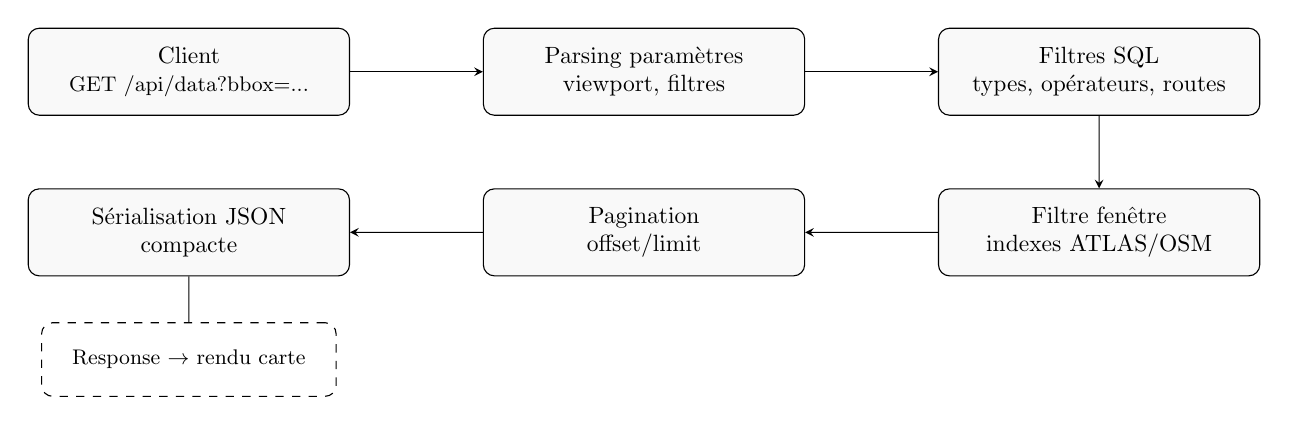
\begin{tikzpicture}[node distance=2.6cm, >=stealth, scale=0.85, every node/.style={transform shape}]
    \tikzstyle{svc}=[draw, rounded corners, minimum width=4.8cm, minimum height=1.3cm, align=center, fill=gray!5]
    \tikzstyle{vol}=[draw, dashed, rounded corners, minimum width=4.4cm, minimum height=1.1cm, align=center, font=\small]

    \node[svc] (client) {Client\\ \small GET /api/data?bbox=...};
    \node[svc, right of=client, node distance=6.8cm] (parse) {Parsing paramètres\\ viewport, filtres};
    \node[svc, right of=parse, node distance=6.8cm] (filters) {Filtres SQL\\ types, opérateurs, routes};
    \node[svc, below of=filters, node distance=2.4cm] (viewport) {Filtre fenêtre\\ indexes ATLAS/OSM};
    \node[svc, left of=viewport, node distance=6.8cm] (paginate) {Pagination\\ offset/limit};
    \node[svc, left of=paginate, node distance=6.8cm] (serialize) {Sérialisation JSON\\ compacte};

    \draw[->] (client) -- (parse);
    \draw[->] (parse) -- (filters);
    \draw[->] (filters) -- (viewport);
    \draw[->] (viewport) -- (paginate);
    \draw[->] (paginate) -- (serialize);

    \node[vol, below of=serialize, node distance=1.9cm] (resp) {Response \(\rightarrow\) rendu carte};
    \draw[-] (serialize) -- (resp);
  \end{tikzpicture}
  \caption[Flux /api/data]{Pipeline de traitement de \texttt{/api/data}: paramètres \(\rightarrow\) filtres \(\rightarrow\) fenêtre indexée \(\rightarrow\) pagination \(\rightarrow\) JSON.}
\end{figure}

\subsection*{Cycle de persistance des solutions}

\begin{figure}[H]
  \centering
  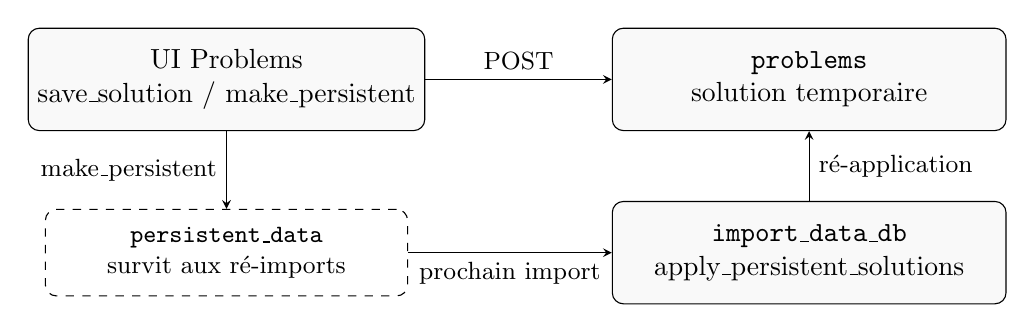
\begin{tikzpicture}[node distance=2.5cm, >=stealth]
    \tikzstyle{svc}=[draw, rounded corners, minimum width=5.0cm, minimum height=1.3cm, align=center, fill=gray!5]
    \tikzstyle{vol}=[draw, dashed, rounded corners, minimum width=4.6cm, minimum height=1.1cm, align=center, font=\small]

    \node[svc] (ui) {UI Problems\\ save\_solution / make\_persistent};
    \node[svc, right of=ui, node distance=7.4cm] (problem) {\texttt{problems}\\ solution temporaire};
    \node[vol, below of=ui, node distance=2.2cm] (persist) {\texttt{persistent\_data}\\ survit aux ré-imports};
    \node[svc, right of=persist, node distance=7.4cm] (import) {\texttt{import\_data\_db}\\ apply\_persistent\_solutions};

    \draw[->] (ui) -- node[above]{\small POST} (problem);
    \draw[->] (ui) -- node[left]{\small make\_persistent} (persist);
    \draw[->] (persist) -- node[below]{\small prochain import} (import);
    \draw[->] (import) -- node[right]{\small ré-application} (problem);
  \end{tikzpicture}
  \caption[Cycle de persistance]{Persistance des solutions/notes: écriture côté API, stockage durable, ré-application au prochain import.}
\end{figure}

\section{Bonnes pratiques et lisibilité}

La maintenabilité du backend repose sur plusieurs principes de conception:

\begin{description}
  \item[Endpoints courts et focalisés] Chaque route a une responsabilité claire et unique. Les blueprints organisent les fonctionnalités par domaine métier.
  
  \item[Paramètres homogènes] Noms stables et prédictibles à travers l'API (ex: \texttt{stop\_filter}, \texttt{match\_method}, \texttt{bbox}) pour simplifier l'intégration côté client.
  
  \item[Sérialisation centralisée] Utilisation systématique de \texttt{format\_stop\_data()} pour éviter la divergence des formats JSON entre endpoints.
  
  \item[Rate limiting défensif] Protection par défaut via \texttt{Limiter} avec réglages fins par route selon la criticité (ex: 30/min pour \texttt{/api/data}, 5/min pour les rapports).
  
  \item[Optimisations anti-patterns] Éviter \texttt{ORDER BY RAND()} sur gros volumes: préférer une sélection pseudo-aléatoire par plage d'ID (cf. \texttt{/api/random\_stop}).
\end{description}

\paragraph{Documentation} Chaque endpoint inclut une docstring explicative pour faciliter la génération automatique de documentation API.

\section*{Et ensuite ?}
Nous approfondirons les mécanismes d'authentification et d'autorisation au \textbf{chapitre 10}, puis l'ensemble du durcissement de la surface d'attaque au \textbf{chapitre 11}. 
